\documentclass[tikz,border=10pt]{standalone}
% No extra TikZ libraries needed.
\begin{document}
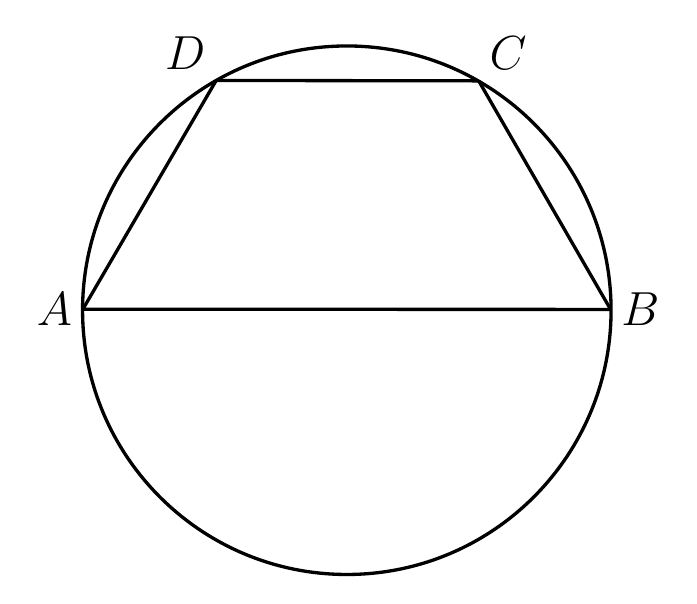
\begin{tikzpicture}[line width=1.2pt, line join=round]
  % Scale s = 0.021333 cm/px (from STYLE METRICS), centre px (224.29, 201.88)
  \coordinate (O) at (0,0);
  \coordinate (A) at (-3.352,0.013);
  \coordinate (B) at (3.350,0.010);
  \coordinate (C) at (1.675,2.913);
  \coordinate (D) at (-1.659,2.918);

  % Circle: centre O, radius 157.28 px * s
  \draw (O) circle (3.356);

  % Chords and diameter
  \draw (A) -- (B);   % diameter AB (through O)
  \draw (D) -- (C);   % horizontal chord DC
  \draw (B) -- (C);
  \draw (A) -- (D);

  % Vertex labels (outside the figure)
  \node[left]        at (A) {\fontsize{17}{20.4}\selectfont $A$};
  \node[right]       at (B) {\fontsize{17}{20.4}\selectfont $B$};
  \node[above right] at (C) {\fontsize{17}{20.4}\selectfont $C$};
  \node[above left]  at (D) {\fontsize{17}{20.4}\selectfont $D$};
\end{tikzpicture}
\end{document}